\documentclass[1p]{elsarticle_modified}
%\bibliographystyle{elsarticle-num}

%\usepackage[colorlinks]{hyperref}
%\usepackage{abbrmath_seonhwa} %\Abb, \Ascr, \Acal ,\Abf, \Afrak
\usepackage{amsfonts}
\usepackage{amssymb}
\usepackage{amsmath}
\usepackage{amsthm}
\usepackage{scalefnt}
\usepackage{amsbsy}
\usepackage{kotex}
\usepackage{caption}
\usepackage{subfig}
\usepackage{color}
\usepackage{graphicx}
\usepackage{xcolor} %% white, black, red, green, blue, cyan, magenta, yellow
\usepackage{float}
\usepackage{setspace}
\usepackage{hyperref}

\usepackage{tikz}
\usetikzlibrary{arrows}

\usepackage{multirow}
\usepackage{array} % fixed length table
\usepackage{hhline}

%%%%%%%%%%%%%%%%%%%%%
\makeatletter
\renewcommand*\env@matrix[1][\arraystretch]{%
	\edef\arraystretch{#1}%
	\hskip -\arraycolsep
	\let\@ifnextchar\new@ifnextchar
	\array{*\c@MaxMatrixCols c}}
\makeatother %https://tex.stackexchange.com/questions/14071/how-can-i-increase-the-line-spacing-in-a-matrix
%%%%%%%%%%%%%%%

\usepackage[normalem]{ulem}

\newcommand{\msout}[1]{\ifmmode\text{\sout{\ensuremath{#1}}}\else\sout{#1}\fi}
%SOURCE: \msout is \stkout macro in https://tex.stackexchange.com/questions/20609/strikeout-in-math-mode

\newcommand{\cancel}[1]{
	\ifmmode
	{\color{red}\msout{#1}}
	\else
	{\color{red}\sout{#1}}
	\fi
}

\newcommand{\add}[1]{
	{\color{blue}\uwave{#1}}
}

\newcommand{\replace}[2]{
	\ifmmode
	{\color{red}\msout{#1}}{\color{blue}\uwave{#2}}
	\else
	{\color{red}\sout{#1}}{\color{blue}\uwave{#2}}
	\fi
}

\newcommand{\Sol}{\mathcal{S}} %segment
\newcommand{\D}{D} %diagram
\newcommand{\A}{\mathcal{A}} %arc


%%%%%%%%%%%%%%%%%%%%%%%%%%%%%5 test

\def\sl{\operatorname{\textup{SL}}(2,\Cbb)}
\def\psl{\operatorname{\textup{PSL}}(2,\Cbb)}
\def\quan{\mkern 1mu \triangleright \mkern 1mu}

\theoremstyle{definition}
\newtheorem{thm}{Theorem}[section]
\newtheorem{prop}[thm]{Proposition}
\newtheorem{lem}[thm]{Lemma}
\newtheorem{ques}[thm]{Question}
\newtheorem{cor}[thm]{Corollary}
\newtheorem{defn}[thm]{Definition}
\newtheorem{exam}[thm]{Example}
\newtheorem{rmk}[thm]{Remark}
\newtheorem{alg}[thm]{Algorithm}

\newcommand{\I}{\sqrt{-1}}
\begin{document}

%\begin{frontmatter}
%
%\title{Boundary parabolic representations of knots up to 8 crossings}
%
%%% Group authors per affiliation:
%\author{Yunhi Cho} 
%\address{Department of Mathematics, University of Seoul, Seoul, Korea}
%\ead{yhcho@uos.ac.kr}
%
%
%\author{Seonhwa Kim} %\fnref{s_kim}}
%\address{Center for Geometry and Physics, Institute for Basic Science, Pohang, 37673, Korea}
%\ead{ryeona17@ibs.re.kr}
%
%\author{Hyuk Kim}
%\address{Department of Mathematical Sciences, Seoul National University, Seoul 08826, Korea}
%\ead{hyukkim@snu.ac.kr}
%
%\author{Seokbeom Yoon}
%\address{Department of Mathematical Sciences, Seoul National University, Seoul, 08826,  Korea}
%\ead{sbyoon15@snu.ac.kr}
%
%\begin{abstract}
%We find all boundary parabolic representation of knots up to 8 crossings.
%
%\end{abstract}
%\begin{keyword}
%    \MSC[2010] 57M25 
%\end{keyword}
%
%\end{frontmatter}

%\linenumbers
%\tableofcontents
%
\newcommand\colored[1]{\textcolor{white}{\rule[-0.35ex]{0.8em}{1.4ex}}\kern-0.8em\color{red} #1}%
%\newcommand\colored[1]{\textcolor{white}{ #1}\kern-2.17ex	\textcolor{white}{ #1}\kern-1.81ex	\textcolor{white}{ #1}\kern-2.15ex\color{red}#1	}

{\Large $\underline{12n_{0597}~(K12n_{0597})}$}

\setlength{\tabcolsep}{10pt}
\renewcommand{\arraystretch}{1.6}
\vspace{1cm}\begin{tabular}{m{100pt}>{\centering\arraybackslash}m{274pt}}
\multirow{5}{120pt}{
	\centering
	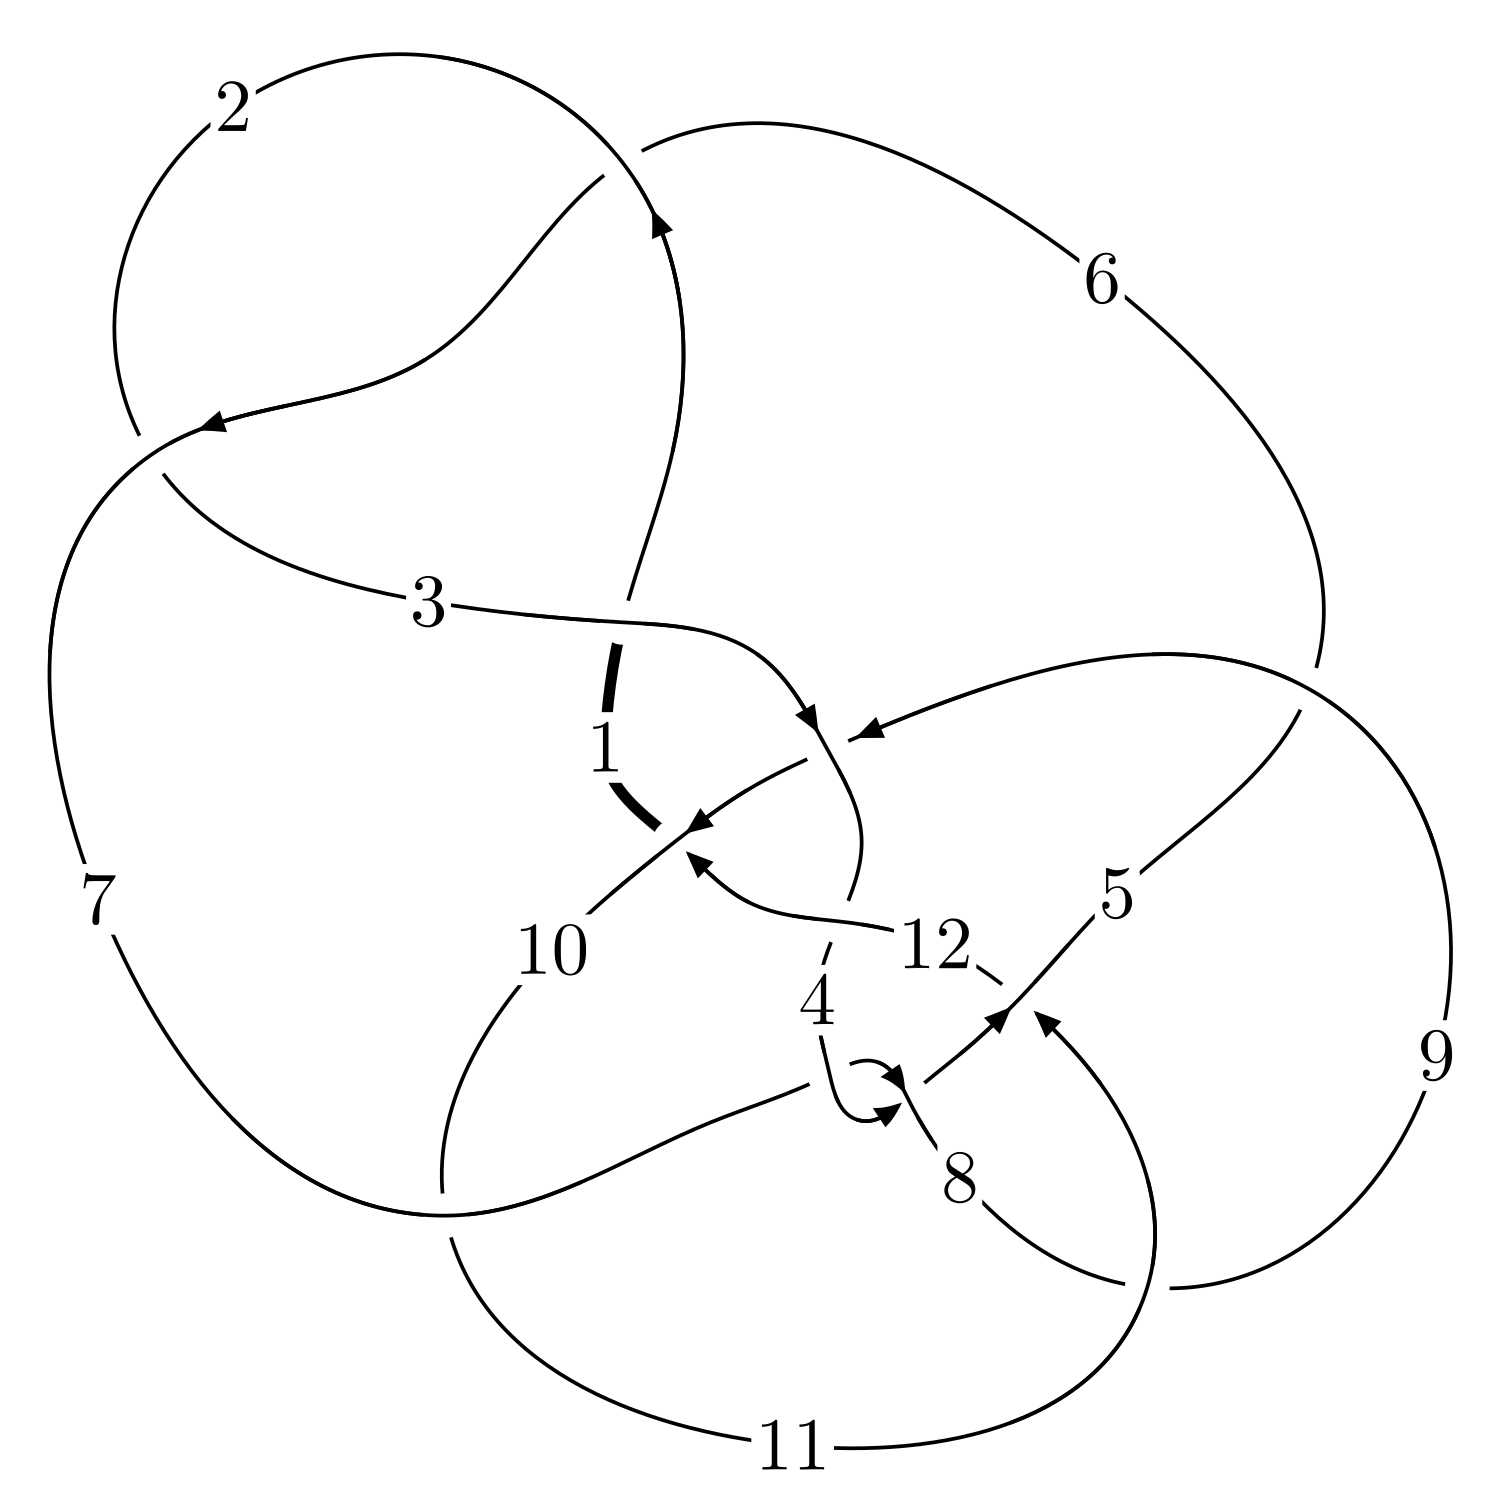
\includegraphics[width=112pt]{../../../GIT/diagram.site/Diagrams/png/2686_12n_0597.png}\\
\ \ \ A knot diagram\footnotemark}&
\allowdisplaybreaks
\textbf{Linearized knot diagam} \\
\cline{2-2}
 &
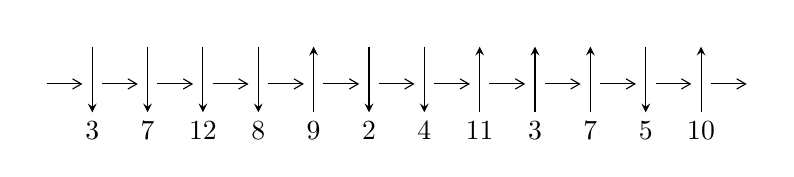
\begin{tikzpicture}[x=20pt, y=17pt]
	% nodes
	\node (C0) at (0, 0) {};
	\node (C1) at (1, 0) {};
	\node (C1U) at (1, +1) {};
	\node (C1D) at (1, -1) {3};

	\node (C2) at (2, 0) {};
	\node (C2U) at (2, +1) {};
	\node (C2D) at (2, -1) {7};

	\node (C3) at (3, 0) {};
	\node (C3U) at (3, +1) {};
	\node (C3D) at (3, -1) {12};

	\node (C4) at (4, 0) {};
	\node (C4U) at (4, +1) {};
	\node (C4D) at (4, -1) {8};

	\node (C5) at (5, 0) {};
	\node (C5U) at (5, +1) {};
	\node (C5D) at (5, -1) {9};

	\node (C6) at (6, 0) {};
	\node (C6U) at (6, +1) {};
	\node (C6D) at (6, -1) {2};

	\node (C7) at (7, 0) {};
	\node (C7U) at (7, +1) {};
	\node (C7D) at (7, -1) {4};

	\node (C8) at (8, 0) {};
	\node (C8U) at (8, +1) {};
	\node (C8D) at (8, -1) {11};

	\node (C9) at (9, 0) {};
	\node (C9U) at (9, +1) {};
	\node (C9D) at (9, -1) {3};

	\node (C10) at (10, 0) {};
	\node (C10U) at (10, +1) {};
	\node (C10D) at (10, -1) {7};

	\node (C11) at (11, 0) {};
	\node (C11U) at (11, +1) {};
	\node (C11D) at (11, -1) {5};

	\node (C12) at (12, 0) {};
	\node (C12U) at (12, +1) {};
	\node (C12D) at (12, -1) {10};
	\node (C13) at (13, 0) {};

	% arrows
	\draw[->,>={angle 60}]
	(C0) edge (C1) (C1) edge (C2) (C2) edge (C3) (C3) edge (C4) (C4) edge (C5) (C5) edge (C6) (C6) edge (C7) (C7) edge (C8) (C8) edge (C9) (C9) edge (C10) (C10) edge (C11) (C11) edge (C12) (C12) edge (C13) ;	\draw[->,>=stealth]
	(C1U) edge (C1D) (C2U) edge (C2D) (C3U) edge (C3D) (C4U) edge (C4D) (C5D) edge (C5U) (C6U) edge (C6D) (C7U) edge (C7D) (C8D) edge (C8U) (C9D) edge (C9U) (C10D) edge (C10U) (C11U) edge (C11D) (C12D) edge (C12U) ;
	\end{tikzpicture} \\
\hhline{~~} \\& 
\textbf{Solving Sequence} \\ \cline{2-2} 
 &
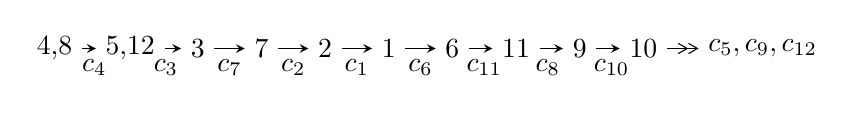
\begin{tikzpicture}[x=23pt, y=7pt]
	% node
	\node (A0) at (-1/8, 0) {4,8};
	\node (A1) at (17/16, 0) {5,12};
	\node (A2) at (17/8, 0) {3};
	\node (A3) at (25/8, 0) {7};
	\node (A4) at (33/8, 0) {2};
	\node (A5) at (41/8, 0) {1};
	\node (A6) at (49/8, 0) {6};
	\node (A7) at (57/8, 0) {11};
	\node (A8) at (65/8, 0) {9};
	\node (A9) at (73/8, 0) {10};
	\node (C1) at (1/2, -1) {$c_{4}$};
	\node (C2) at (13/8, -1) {$c_{3}$};
	\node (C3) at (21/8, -1) {$c_{7}$};
	\node (C4) at (29/8, -1) {$c_{2}$};
	\node (C5) at (37/8, -1) {$c_{1}$};
	\node (C6) at (45/8, -1) {$c_{6}$};
	\node (C7) at (53/8, -1) {$c_{11}$};
	\node (C8) at (61/8, -1) {$c_{8}$};
	\node (C9) at (69/8, -1) {$c_{10}$};
	\node (A10) at (11, 0) {$c_{5},c_{9},c_{12}$};

	% edge
	\draw[->,>=stealth]	
	(A0) edge (A1) (A1) edge (A2) (A2) edge (A3) (A3) edge (A4) (A4) edge (A5) (A5) edge (A6) (A6) edge (A7) (A7) edge (A8) (A8) edge (A9) ;
	\draw[->>,>={angle 60}]	
	(A9) edge (A10);
\end{tikzpicture} \\ 

\end{tabular} \\

\footnotetext{
The image of knot diagram is generated by the software ``\textbf{Draw programme}" developed by Andrew Bartholomew(\url{http://www.layer8.co.uk/maths/draw/index.htm\#Running-draw}), where we modified some parts for our purpose(\url{https://github.com/CATsTAILs/LinksPainter}).
}\phantom \\ \newline 
\centering \textbf{Ideals for irreducible components\footnotemark of $X_{\text{par}}$} 
 
\begin{align*}
I^u_{1}&=\langle 
6.48488\times10^{68} u^{54}+2.22735\times10^{69} u^{53}+\cdots+3.01163\times10^{67} b-4.54938\times10^{69},\\
\phantom{I^u_{1}}&\phantom{= \langle  }7.79191\times10^{69} u^{54}+2.67697\times10^{70} u^{53}+\cdots+6.02326\times10^{67} a-5.52191\times10^{70},\;u^{55}+4 u^{54}+\cdots-32 u-4\rangle \\
I^u_{2}&=\langle 
1742938 u^{19}+1162593 u^{18}+\cdots+1826407 b+1460687,\\
\phantom{I^u_{2}}&\phantom{= \langle  }147076 u^{19}+1158 u^{18}+\cdots+166037 a-623712,\;u^{20}+u^{19}+\cdots-4 u+1\rangle \\
I^u_{3}&=\langle 
- a^3+b+2 a+1,\;a^4- a^3-4 a^2+2 a+5,\;u-1\rangle \\
I^u_{4}&=\langle 
b-1,\;a-1,\;u-1\rangle \\
I^u_{5}&=\langle 
b- u+1,\;u^2+a-2 u+1,\;u^3- u^2+1\rangle \\
\\
\end{align*}
\raggedright * 5 irreducible components of $\dim_{\mathbb{C}}=0$, with total 83 representations.\\
\footnotetext{All coefficients of polynomials are rational numbers. But the coefficients are sometimes approximated in decimal forms when there is not enough margin.}
\newpage
\renewcommand{\arraystretch}{1}
\centering \section*{I. $I^u_{1}= \langle 6.48\times10^{68} u^{54}+2.23\times10^{69} u^{53}+\cdots+3.01\times10^{67} b-4.55\times10^{69},\;7.79\times10^{69} u^{54}+2.68\times10^{70} u^{53}+\cdots+6.02\times10^{67} a-5.52\times10^{70},\;u^{55}+4 u^{54}+\cdots-32 u-4 \rangle$}
\flushleft \textbf{(i) Arc colorings}\\
\begin{tabular}{m{7pt} m{180pt} m{7pt} m{180pt} }
\flushright $a_{4}=$&$\begin{pmatrix}1\\0\end{pmatrix}$ \\
\flushright $a_{8}=$&$\begin{pmatrix}0\\u\end{pmatrix}$ \\
\flushright $a_{5}=$&$\begin{pmatrix}1\\u^2\end{pmatrix}$ \\
\flushright $a_{12}=$&$\begin{pmatrix}-129.364 u^{54}-444.439 u^{53}+\cdots+5697.58 u+916.764\\-21.5328 u^{54}-73.9584 u^{53}+\cdots+941.610 u+151.061\end{pmatrix}$ \\
\flushright $a_{3}=$&$\begin{pmatrix}3.94666 u^{54}+13.1180 u^{53}+\cdots-136.672 u-18.8314\\-20.4560 u^{54}-70.0814 u^{53}+\cdots+894.192 u+143.944\end{pmatrix}$ \\
\flushright $a_{7}=$&$\begin{pmatrix}u\\u\end{pmatrix}$ \\
\flushright $a_{2}=$&$\begin{pmatrix}-4.54849 u^{54}-15.8254 u^{53}+\cdots+226.873 u+38.8130\\-28.9511 u^{54}-99.0248 u^{53}+\cdots+1257.74 u+201.588\end{pmatrix}$ \\
\flushright $a_{1}=$&$\begin{pmatrix}-172.432 u^{54}-590.262 u^{53}+\cdots+7505.58 u+1199.19\\40.4434 u^{54}+139.041 u^{53}+\cdots-1788.25 u-286.747\end{pmatrix}$ \\
\flushright $a_{6}=$&$\begin{pmatrix}-20.9960 u^{54}-71.3826 u^{53}+\cdots+880.148 u+137.913\\66.7999 u^{54}+229.120 u^{53}+\cdots-2923.17 u-468.173\end{pmatrix}$ \\
\flushright $a_{11}=$&$\begin{pmatrix}-109.774 u^{54}-377.006 u^{53}+\cdots+4820.14 u+775.762\\-15.4249 u^{54}-52.9241 u^{53}+\cdots+670.322 u+107.355\end{pmatrix}$ \\
\flushright $a_{9}=$&$\begin{pmatrix}190.838 u^{54}+654.783 u^{53}+\cdots-8370.59 u-1338.55\\-44.5724 u^{54}-152.962 u^{53}+\cdots+1958.63 u+314.711\end{pmatrix}$ \\
\flushright $a_{10}=$&$\begin{pmatrix}-139.838 u^{54}-480.350 u^{53}+\cdots+6148.79 u+989.017\\-45.4892 u^{54}-156.268 u^{53}+\cdots+1998.97 u+320.610\end{pmatrix}$\\&\end{tabular}
\flushleft \textbf{(ii) Obstruction class $= -1$}\\~\\
\flushleft \textbf{(iii) Cusp Shapes $= -41.4839 u^{54}-141.696 u^{53}+\cdots+1753.72 u+276.705$}\\~\\
\newpage\renewcommand{\arraystretch}{1}
\flushleft \textbf{(iv) u-Polynomials at the component}\newline \\
\begin{tabular}{m{50pt}|m{274pt}}
Crossings & \hspace{64pt}u-Polynomials at each crossing \\
\hline $$\begin{aligned}c_{1}\end{aligned}$$&$\begin{aligned}
&u^{55}+84 u^{54}+\cdots-72 u+1
\end{aligned}$\\
\hline $$\begin{aligned}c_{2},c_{6}\end{aligned}$$&$\begin{aligned}
&u^{55}-2 u^{54}+\cdots+22 u-1
\end{aligned}$\\
\hline $$\begin{aligned}c_{3}\end{aligned}$$&$\begin{aligned}
&u^{55}-8 u^{54}+\cdots-120 u+25
\end{aligned}$\\
\hline $$\begin{aligned}c_{4},c_{7}\end{aligned}$$&$\begin{aligned}
&u^{55}-4 u^{54}+\cdots-32 u+4
\end{aligned}$\\
\hline $$\begin{aligned}c_{5}\end{aligned}$$&$\begin{aligned}
&u^{55}-3 u^{54}+\cdots+75901 u-173113
\end{aligned}$\\
\hline $$\begin{aligned}c_{8}\end{aligned}$$&$\begin{aligned}
&u^{55}+10 u^{54}+\cdots-1715 u-229
\end{aligned}$\\
\hline $$\begin{aligned}c_{9}\end{aligned}$$&$\begin{aligned}
&u^{55}- u^{54}+\cdots-216467 u+35417
\end{aligned}$\\
\hline $$\begin{aligned}c_{10}\end{aligned}$$&$\begin{aligned}
&u^{55}-4 u^{54}+\cdots-936251 u-118509
\end{aligned}$\\
\hline $$\begin{aligned}c_{11}\end{aligned}$$&$\begin{aligned}
&u^{55}+2 u^{54}+\cdots+4 u-24
\end{aligned}$\\
\hline $$\begin{aligned}c_{12}\end{aligned}$$&$\begin{aligned}
&u^{55}- u^{54}+\cdots+3199358 u-321516
\end{aligned}$\\
\hline
\end{tabular}\\~\\
\newpage\renewcommand{\arraystretch}{1}
\flushleft \textbf{(v) Riley Polynomials at the component}\newline \\
\begin{tabular}{m{50pt}|m{274pt}}
Crossings & \hspace{64pt}Riley Polynomials at each crossing \\
\hline $$\begin{aligned}c_{1}\end{aligned}$$&$\begin{aligned}
&y^{55}-212 y^{54}+\cdots+10440 y-1
\end{aligned}$\\
\hline $$\begin{aligned}c_{2},c_{6}\end{aligned}$$&$\begin{aligned}
&y^{55}-84 y^{54}+\cdots-72 y-1
\end{aligned}$\\
\hline $$\begin{aligned}c_{3}\end{aligned}$$&$\begin{aligned}
&y^{55}+20 y^{54}+\cdots-800 y-625
\end{aligned}$\\
\hline $$\begin{aligned}c_{4},c_{7}\end{aligned}$$&$\begin{aligned}
&y^{55}-36 y^{54}+\cdots-200 y-16
\end{aligned}$\\
\hline $$\begin{aligned}c_{5}\end{aligned}$$&$\begin{aligned}
&y^{55}+35 y^{54}+\cdots+119306470953 y-29968110769
\end{aligned}$\\
\hline $$\begin{aligned}c_{8}\end{aligned}$$&$\begin{aligned}
&y^{55}+20 y^{54}+\cdots-2180589 y-52441
\end{aligned}$\\
\hline $$\begin{aligned}c_{9}\end{aligned}$$&$\begin{aligned}
&y^{55}+91 y^{54}+\cdots+50901662647 y-1254363889
\end{aligned}$\\
\hline $$\begin{aligned}c_{10}\end{aligned}$$&$\begin{aligned}
&y^{55}+58 y^{54}+\cdots-129372587591 y-14044383081
\end{aligned}$\\
\hline $$\begin{aligned}c_{11}\end{aligned}$$&$\begin{aligned}
&y^{55}-6 y^{54}+\cdots-12656 y-576
\end{aligned}$\\
\hline $$\begin{aligned}c_{12}\end{aligned}$$&$\begin{aligned}
&y^{55}+85 y^{54}+\cdots+3623181372652 y-103372538256
\end{aligned}$\\
\hline
\end{tabular}\\~\\
\newpage\flushleft \textbf{(vi) Complex Volumes and Cusp Shapes}
$$\begin{array}{c|c|c}  
\text{Solutions to }I^u_{1}& \I (\text{vol} + \sqrt{-1}CS) & \text{Cusp shape}\\
 \hline 
\begin{aligned}
u &= -0.228394 + 0.930097 I \\
a &= -0.355410 + 0.174211 I \\
b &= -0.216207 - 0.780987 I\end{aligned}
 & \phantom{-}2.63763 - 2.19314 I & \phantom{-}0.766014 + 1.147808 I \\ \hline\begin{aligned}
u &= -0.228394 - 0.930097 I \\
a &= -0.355410 - 0.174211 I \\
b &= -0.216207 + 0.780987 I\end{aligned}
 & \phantom{-}2.63763 + 2.19314 I & \phantom{-}0.766014 - 1.147808 I \\ \hline\begin{aligned}
u &= -0.061115 + 1.061790 I \\
a &= \phantom{-}0.121223 - 0.494313 I \\
b &= \phantom{-}0.396675 + 1.163810 I\end{aligned}
 & \phantom{-}1.55867 - 3.48219 I & \phantom{-0.000000 -}0. + 3.47906 I \\ \hline\begin{aligned}
u &= -0.061115 - 1.061790 I \\
a &= \phantom{-}0.121223 + 0.494313 I \\
b &= \phantom{-}0.396675 - 1.163810 I\end{aligned}
 & \phantom{-}1.55867 + 3.48219 I & \phantom{-0.000000 } 0. - 3.47906 I \\ \hline\begin{aligned}
u &= \phantom{-}1.013150 + 0.429080 I \\
a &= -2.09376 - 0.07084 I \\
b &= -1.30226 - 1.21278 I\end{aligned}
 & -8.91481 - 6.34317 I & \phantom{-0.000000 } 0 \\ \hline\begin{aligned}
u &= \phantom{-}1.013150 - 0.429080 I \\
a &= -2.09376 + 0.07084 I \\
b &= -1.30226 + 1.21278 I\end{aligned}
 & -8.91481 + 6.34317 I & \phantom{-0.000000 } 0 \\ \hline\begin{aligned}
u &= -1.079130 + 0.236177 I \\
a &= \phantom{-}1.53166 - 0.57910 I \\
b &= \phantom{-}0.77564 - 1.31217 I\end{aligned}
 & -1.46530 + 4.21934 I & \phantom{-0.000000 } 0 \\ \hline\begin{aligned}
u &= -1.079130 - 0.236177 I \\
a &= \phantom{-}1.53166 + 0.57910 I \\
b &= \phantom{-}0.77564 + 1.31217 I\end{aligned}
 & -1.46530 - 4.21934 I & \phantom{-0.000000 } 0 \\ \hline\begin{aligned}
u &= -1.113000 + 0.147678 I \\
a &= -1.55961 - 0.95086 I \\
b &= -0.546370 + 1.079590 I\end{aligned}
 & -12.12370 + 4.63839 I & \phantom{-0.000000 } 0 \\ \hline\begin{aligned}
u &= -1.113000 - 0.147678 I \\
a &= -1.55961 + 0.95086 I \\
b &= -0.546370 - 1.079590 I\end{aligned}
 & -12.12370 - 4.63839 I & \phantom{-0.000000 } 0\\
 \hline 
 \end{array}$$\newpage$$\begin{array}{c|c|c}  
\text{Solutions to }I^u_{1}& \I (\text{vol} + \sqrt{-1}CS) & \text{Cusp shape}\\
 \hline 
\begin{aligned}
u &= -0.398648 + 0.764365 I \\
a &= \phantom{-}0.490007 + 1.105910 I \\
b &= -0.751133 - 0.461027 I\end{aligned}
 & -10.69800 + 3.28061 I & -4.43813 - 2.05243 I \\ \hline\begin{aligned}
u &= -0.398648 - 0.764365 I \\
a &= \phantom{-}0.490007 - 1.105910 I \\
b &= -0.751133 + 0.461027 I\end{aligned}
 & -10.69800 - 3.28061 I & -4.43813 + 2.05243 I \\ \hline\begin{aligned}
u &= -0.818436 + 0.220706 I \\
a &= -0.462335 - 0.757558 I \\
b &= -0.258171 - 1.314110 I\end{aligned}
 & \phantom{-}1.02370 + 2.96901 I & \phantom{-}6.22160 - 5.57360 I \\ \hline\begin{aligned}
u &= -0.818436 - 0.220706 I \\
a &= -0.462335 + 0.757558 I \\
b &= -0.258171 + 1.314110 I\end{aligned}
 & \phantom{-}1.02370 - 2.96901 I & \phantom{-}6.22160 + 5.57360 I \\ \hline\begin{aligned}
u &= \phantom{-}0.823693\phantom{ +0.000000I} \\
a &= \phantom{-}2.96416\phantom{ +0.000000I} \\
b &= \phantom{-}1.33894\phantom{ +0.000000I}\end{aligned}
 & -0.453310\phantom{ +0.000000I} & -12.4430\phantom{ +0.000000I} \\ \hline\begin{aligned}
u &= \phantom{-}0.629407 + 1.015120 I \\
a &= -0.124519 + 0.360519 I \\
b &= \phantom{-}0.354817 - 0.497624 I\end{aligned}
 & -0.865641 - 0.009239 I & \phantom{-0.000000 } 0 \\ \hline\begin{aligned}
u &= \phantom{-}0.629407 - 1.015120 I \\
a &= -0.124519 - 0.360519 I \\
b &= \phantom{-}0.354817 + 0.497624 I\end{aligned}
 & -0.865641 + 0.009239 I & \phantom{-0.000000 } 0 \\ \hline\begin{aligned}
u &= \phantom{-}0.056692 + 1.212890 I \\
a &= -0.103950 - 0.233463 I \\
b &= -0.682228 + 1.128040 I\end{aligned}
 & -8.74789 + 8.87696 I & \phantom{-0.000000 } 0 \\ \hline\begin{aligned}
u &= \phantom{-}0.056692 - 1.212890 I \\
a &= -0.103950 + 0.233463 I \\
b &= -0.682228 - 1.128040 I\end{aligned}
 & -8.74789 - 8.87696 I & \phantom{-0.000000 } 0 \\ \hline\begin{aligned}
u &= \phantom{-}0.354907 + 0.697158 I \\
a &= -0.098793 - 0.883310 I \\
b &= \phantom{-}0.155774 + 1.110550 I\end{aligned}
 & \phantom{-}2.01009 - 2.16153 I & \phantom{-}2.20037 + 5.52786 I\\
 \hline 
 \end{array}$$\newpage$$\begin{array}{c|c|c}  
\text{Solutions to }I^u_{1}& \I (\text{vol} + \sqrt{-1}CS) & \text{Cusp shape}\\
 \hline 
\begin{aligned}
u &= \phantom{-}0.354907 - 0.697158 I \\
a &= -0.098793 + 0.883310 I \\
b &= \phantom{-}0.155774 - 1.110550 I\end{aligned}
 & \phantom{-}2.01009 + 2.16153 I & \phantom{-}2.20037 - 5.52786 I \\ \hline\begin{aligned}
u &= \phantom{-}0.388472 + 0.676966 I \\
a &= \phantom{-}0.392074 + 0.586948 I \\
b &= -0.77671 + 1.19630 I\end{aligned}
 & -7.10371 + 2.13418 I & -1.61598 - 0.45444 I \\ \hline\begin{aligned}
u &= \phantom{-}0.388472 - 0.676966 I \\
a &= \phantom{-}0.392074 - 0.586948 I \\
b &= -0.77671 - 1.19630 I\end{aligned}
 & -7.10371 - 2.13418 I & -1.61598 + 0.45444 I \\ \hline\begin{aligned}
u &= \phantom{-}1.169370 + 0.406827 I \\
a &= \phantom{-}0.160942 - 0.680261 I \\
b &= \phantom{-}0.558665 - 1.106950 I\end{aligned}
 & -2.81126 - 1.20544 I & \phantom{-0.000000 } 0 \\ \hline\begin{aligned}
u &= \phantom{-}1.169370 - 0.406827 I \\
a &= \phantom{-}0.160942 + 0.680261 I \\
b &= \phantom{-}0.558665 + 1.106950 I\end{aligned}
 & -2.81126 + 1.20544 I & \phantom{-0.000000 } 0 \\ \hline\begin{aligned}
u &= -1.256970 + 0.280156 I \\
a &= \phantom{-}1.366380 + 0.304132 I \\
b &= \phantom{-}1.164040 + 0.121414 I\end{aligned}
 & -6.24743 + 2.95707 I & \phantom{-0.000000 } 0 \\ \hline\begin{aligned}
u &= -1.256970 - 0.280156 I \\
a &= \phantom{-}1.366380 - 0.304132 I \\
b &= \phantom{-}1.164040 - 0.121414 I\end{aligned}
 & -6.24743 - 2.95707 I & \phantom{-0.000000 } 0 \\ \hline\begin{aligned}
u &= \phantom{-}1.247720 + 0.445260 I \\
a &= -1.217490 - 0.284802 I \\
b &= -0.241125 - 0.911262 I\end{aligned}
 & -1.00747 - 2.30946 I & \phantom{-0.000000 } 0 \\ \hline\begin{aligned}
u &= \phantom{-}1.247720 - 0.445260 I \\
a &= -1.217490 + 0.284802 I \\
b &= -0.241125 + 0.911262 I\end{aligned}
 & -1.00747 + 2.30946 I & \phantom{-0.000000 } 0 \\ \hline\begin{aligned}
u &= \phantom{-}1.283620 + 0.343428 I \\
a &= -1.33294 + 0.59936 I \\
b &= -1.55960 + 0.59836 I\end{aligned}
 & -15.4853 - 6.9210 I & \phantom{-0.000000 } 0\\
 \hline 
 \end{array}$$\newpage$$\begin{array}{c|c|c}  
\text{Solutions to }I^u_{1}& \I (\text{vol} + \sqrt{-1}CS) & \text{Cusp shape}\\
 \hline 
\begin{aligned}
u &= \phantom{-}1.283620 - 0.343428 I \\
a &= -1.33294 - 0.59936 I \\
b &= -1.55960 - 0.59836 I\end{aligned}
 & -15.4853 + 6.9210 I & \phantom{-0.000000 } 0 \\ \hline\begin{aligned}
u &= \phantom{-}1.318640 + 0.262440 I \\
a &= \phantom{-}1.39643 + 0.81108 I \\
b &= \phantom{-}0.598048 + 0.736018 I\end{aligned}
 & -3.05878 - 4.93696 I & \phantom{-0.000000 } 0 \\ \hline\begin{aligned}
u &= \phantom{-}1.318640 - 0.262440 I \\
a &= \phantom{-}1.39643 - 0.81108 I \\
b &= \phantom{-}0.598048 - 0.736018 I\end{aligned}
 & -3.05878 + 4.93696 I & \phantom{-0.000000 } 0 \\ \hline\begin{aligned}
u &= -1.254450 + 0.537906 I \\
a &= -1.361600 + 0.016121 I \\
b &= -0.644516 + 0.771416 I\end{aligned}
 & -0.61529 + 7.55097 I & \phantom{-0.000000 } 0 \\ \hline\begin{aligned}
u &= -1.254450 - 0.537906 I \\
a &= -1.361600 - 0.016121 I \\
b &= -0.644516 - 0.771416 I\end{aligned}
 & -0.61529 - 7.55097 I & \phantom{-0.000000 } 0 \\ \hline\begin{aligned}
u &= \phantom{-}0.543362 + 0.279828 I \\
a &= -0.184351 + 0.678862 I \\
b &= \phantom{-}0.386325 + 0.158096 I\end{aligned}
 & -1.238630 - 0.333157 I & -8.21440 + 1.77959 I \\ \hline\begin{aligned}
u &= \phantom{-}0.543362 - 0.279828 I \\
a &= -0.184351 - 0.678862 I \\
b &= \phantom{-}0.386325 - 0.158096 I\end{aligned}
 & -1.238630 + 0.333157 I & -8.21440 - 1.77959 I \\ \hline\begin{aligned}
u &= -0.532879 + 0.265595 I \\
a &= -1.87909 - 0.15769 I \\
b &= -0.496585 + 0.280323 I\end{aligned}
 & \phantom{-}1.53458 - 0.08260 I & \phantom{-}8.02360 - 0.70539 I \\ \hline\begin{aligned}
u &= -0.532879 - 0.265595 I \\
a &= -1.87909 + 0.15769 I \\
b &= -0.496585 - 0.280323 I\end{aligned}
 & \phantom{-}1.53458 + 0.08260 I & \phantom{-}8.02360 + 0.70539 I \\ \hline\begin{aligned}
u &= -1.211180 + 0.728080 I \\
a &= -0.875893 - 0.683728 I \\
b &= -0.631732 + 1.072700 I\end{aligned}
 & -12.79060 + 2.58251 I & \phantom{-0.000000 } 0\\
 \hline 
 \end{array}$$\newpage$$\begin{array}{c|c|c}  
\text{Solutions to }I^u_{1}& \I (\text{vol} + \sqrt{-1}CS) & \text{Cusp shape}\\
 \hline 
\begin{aligned}
u &= -1.211180 - 0.728080 I \\
a &= -0.875893 + 0.683728 I \\
b &= -0.631732 - 1.072700 I\end{aligned}
 & -12.79060 - 2.58251 I & \phantom{-0.000000 } 0 \\ \hline\begin{aligned}
u &= \phantom{-}1.25664 + 0.67520 I \\
a &= \phantom{-}1.073550 - 0.367845 I \\
b &= \phantom{-}0.700106 + 0.896451 I\end{aligned}
 & -3.21944 - 6.43186 I & \phantom{-0.000000 } 0 \\ \hline\begin{aligned}
u &= \phantom{-}1.25664 - 0.67520 I \\
a &= \phantom{-}1.073550 + 0.367845 I \\
b &= \phantom{-}0.700106 - 0.896451 I\end{aligned}
 & -3.21944 + 6.43186 I & \phantom{-0.000000 } 0 \\ \hline\begin{aligned}
u &= -0.568585 + 0.002353 I \\
a &= \phantom{-}2.93796 + 2.07601 I \\
b &= -0.463493 + 0.346007 I\end{aligned}
 & -10.21720 + 3.48231 I & -4.98199 + 0.62812 I \\ \hline\begin{aligned}
u &= -0.568585 - 0.002353 I \\
a &= \phantom{-}2.93796 - 2.07601 I \\
b &= -0.463493 - 0.346007 I\end{aligned}
 & -10.21720 - 3.48231 I & -4.98199 - 0.62812 I \\ \hline\begin{aligned}
u &= -1.34385 + 0.51761 I \\
a &= \phantom{-}1.43449 - 0.18164 I \\
b &= \phantom{-}0.60052 - 1.30971 I\end{aligned}
 & -2.54819 + 9.08466 I & \phantom{-0.000000 } 0 \\ \hline\begin{aligned}
u &= -1.34385 - 0.51761 I \\
a &= \phantom{-}1.43449 + 0.18164 I \\
b &= \phantom{-}0.60052 + 1.30971 I\end{aligned}
 & -2.54819 - 9.08466 I & \phantom{-0.000000 } 0 \\ \hline\begin{aligned}
u &= \phantom{-}1.37774 + 0.58999 I \\
a &= -1.49234 - 0.04356 I \\
b &= -0.87943 - 1.33400 I\end{aligned}
 & -12.9172 - 15.1751 I & \phantom{-0.000000 } 0 \\ \hline\begin{aligned}
u &= \phantom{-}1.37774 - 0.58999 I \\
a &= -1.49234 + 0.04356 I \\
b &= -0.87943 + 1.33400 I\end{aligned}
 & -12.9172 + 15.1751 I & \phantom{-0.000000 } 0 \\ \hline\begin{aligned}
u &= -1.50431 + 0.07352 I \\
a &= -0.364764 - 1.062760 I \\
b &= -0.507231 - 0.684175 I\end{aligned}
 & -13.50180 + 0.32367 I & \phantom{-0.000000 } 0\\
 \hline 
 \end{array}$$\newpage$$\begin{array}{c|c|c}  
\text{Solutions to }I^u_{1}& \I (\text{vol} + \sqrt{-1}CS) & \text{Cusp shape}\\
 \hline 
\begin{aligned}
u &= -1.50431 - 0.07352 I \\
a &= -0.364764 + 1.062760 I \\
b &= -0.507231 + 0.684175 I\end{aligned}
 & -13.50180 - 0.32367 I & \phantom{-0.000000 } 0 \\ \hline\begin{aligned}
u &= -1.60007 + 0.48099 I \\
a &= -0.249894 - 0.427368 I \\
b &= -0.631921 - 0.689866 I\end{aligned}
 & -14.0455 - 2.4232 I & \phantom{-0.000000 } 0 \\ \hline\begin{aligned}
u &= -1.60007 - 0.48099 I \\
a &= -0.249894 + 0.427368 I \\
b &= -0.631921 + 0.689866 I\end{aligned}
 & -14.0455 + 2.4232 I & \phantom{-0.000000 } 0 \\ \hline\begin{aligned}
u &= -0.080542 + 0.193890 I \\
a &= \phantom{-}2.61995 - 1.69033 I \\
b &= \phantom{-}0.228619 - 1.091470 I\end{aligned}
 & \phantom{-}1.26586 + 2.57084 I & -0.85088 - 2.32793 I \\ \hline\begin{aligned}
u &= -0.080542 - 0.193890 I \\
a &= \phantom{-}2.61995 + 1.69033 I \\
b &= \phantom{-}0.228619 + 1.091470 I\end{aligned}
 & \phantom{-}1.26586 - 2.57084 I & -0.85088 + 2.32793 I\\
 \hline 
 \end{array}$$\newpage\newpage\renewcommand{\arraystretch}{1}
\centering \section*{II. $I^u_{2}= \langle 1.74\times10^{6} u^{19}+1.16\times10^{6} u^{18}+\cdots+1.83\times10^{6} b+1.46\times10^{6},\;147076 u^{19}+1158 u^{18}+\cdots+166037 a-623712,\;u^{20}+u^{19}+\cdots-4 u+1 \rangle$}
\flushleft \textbf{(i) Arc colorings}\\
\begin{tabular}{m{7pt} m{180pt} m{7pt} m{180pt} }
\flushright $a_{4}=$&$\begin{pmatrix}1\\0\end{pmatrix}$ \\
\flushright $a_{8}=$&$\begin{pmatrix}0\\u\end{pmatrix}$ \\
\flushright $a_{5}=$&$\begin{pmatrix}1\\u^2\end{pmatrix}$ \\
\flushright $a_{12}=$&$\begin{pmatrix}-0.885803 u^{19}-0.00697435 u^{18}+\cdots-0.332149 u+3.75646\\-0.954299 u^{19}-0.636547 u^{18}+\cdots+2.12930 u-0.799760\end{pmatrix}$ \\
\flushright $a_{3}=$&$\begin{pmatrix}-0.167149 u^{19}-0.371082 u^{18}+\cdots-4.30841 u+3.40433\\-0.378146 u^{19}-0.145836 u^{18}+\cdots-2.54026 u+0.496680\end{pmatrix}$ \\
\flushright $a_{7}=$&$\begin{pmatrix}u\\u\end{pmatrix}$ \\
\flushright $a_{2}=$&$\begin{pmatrix}-0.946799 u^{19}-0.655425 u^{18}+\cdots-2.35244 u+2.96809\\-1.15780 u^{19}-0.430180 u^{18}+\cdots-0.584292 u+0.0604367\end{pmatrix}$ \\
\flushright $a_{1}=$&$\begin{pmatrix}-2.36020 u^{19}-0.734061 u^{18}+\cdots+6.88680 u-0.210030\\-1.50970 u^{19}-0.927327 u^{18}+\cdots+5.68923 u-1.07153\end{pmatrix}$ \\
\flushright $a_{6}=$&$\begin{pmatrix}-0.0662196 u^{19}-0.397076 u^{18}+\cdots+1.44845 u+1.51392\\0.193160 u^{19}+0.171997 u^{18}+\cdots+1.73103 u-0.520690\end{pmatrix}$ \\
\flushright $a_{11}=$&$\begin{pmatrix}-1.22425 u^{19}-0.993563 u^{18}+\cdots-2.60396 u+3.83553\\-1.23184 u^{19}-1.39082 u^{18}+\cdots-0.124812 u-0.151619\end{pmatrix}$ \\
\flushright $a_{9}=$&$\begin{pmatrix}-0.119859 u^{19}+0.185423 u^{18}+\cdots-1.51911 u+2.97387\\0.588138 u^{19}+0.846974 u^{18}+\cdots-1.40998 u-0.239062\end{pmatrix}$ \\
\flushright $a_{10}=$&$\begin{pmatrix}-0.807363 u^{19}-0.0873266 u^{18}+\cdots-1.05289 u+3.44587\\-0.814955 u^{19}-0.484584 u^{18}+\cdots+1.42626 u-0.541284\end{pmatrix}$\\&\end{tabular}
\flushleft \textbf{(ii) Obstruction class $= 1$}\\~\\
\flushleft \textbf{(iii) Cusp Shapes $= \frac{3759113}{1826407} u^{19}+\frac{9918792}{1826407} u^{18}+\cdots+\frac{33892975}{1826407} u-\frac{13352398}{1826407}$}\\~\\
\newpage\renewcommand{\arraystretch}{1}
\flushleft \textbf{(iv) u-Polynomials at the component}\newline \\
\begin{tabular}{m{50pt}|m{274pt}}
Crossings & \hspace{64pt}u-Polynomials at each crossing \\
\hline $$\begin{aligned}c_{1}\end{aligned}$$&$\begin{aligned}
&u^{20}-22 u^{19}+\cdots-3 u+1
\end{aligned}$\\
\hline $$\begin{aligned}c_{2}\end{aligned}$$&$\begin{aligned}
&u^{20}+2 u^{19}+\cdots- u+1
\end{aligned}$\\
\hline $$\begin{aligned}c_{3}\end{aligned}$$&$\begin{aligned}
&u^{20}+5 u^{19}+\cdots+5 u+1
\end{aligned}$\\
\hline $$\begin{aligned}c_{4}\end{aligned}$$&$\begin{aligned}
&u^{20}+u^{19}+\cdots-4 u+1
\end{aligned}$\\
\hline $$\begin{aligned}c_{5}\end{aligned}$$&$\begin{aligned}
&u^{20}- u^{19}+\cdots+5 u+1
\end{aligned}$\\
\hline $$\begin{aligned}c_{6}\end{aligned}$$&$\begin{aligned}
&u^{20}-2 u^{19}+\cdots+u+1
\end{aligned}$\\
\hline $$\begin{aligned}c_{7}\end{aligned}$$&$\begin{aligned}
&u^{20}- u^{19}+\cdots+4 u+1
\end{aligned}$\\
\hline $$\begin{aligned}c_{8}\end{aligned}$$&$\begin{aligned}
&u^{20}+6 u^{19}+\cdots+u+1
\end{aligned}$\\
\hline $$\begin{aligned}c_{9}\end{aligned}$$&$\begin{aligned}
&u^{20}- u^{19}+\cdots+9 u+1
\end{aligned}$\\
\hline $$\begin{aligned}c_{10}\end{aligned}$$&$\begin{aligned}
&u^{20}+6 u^{19}+\cdots+62 u+25
\end{aligned}$\\
\hline $$\begin{aligned}c_{11}\end{aligned}$$&$\begin{aligned}
&u^{20}+u^{19}+\cdots-24 u+23
\end{aligned}$\\
\hline $$\begin{aligned}c_{12}\end{aligned}$$&$\begin{aligned}
&u^{20}- u^{19}+\cdots+3 u+1
\end{aligned}$\\
\hline
\end{tabular}\\~\\
\newpage\renewcommand{\arraystretch}{1}
\flushleft \textbf{(v) Riley Polynomials at the component}\newline \\
\begin{tabular}{m{50pt}|m{274pt}}
Crossings & \hspace{64pt}Riley Polynomials at each crossing \\
\hline $$\begin{aligned}c_{1}\end{aligned}$$&$\begin{aligned}
&y^{20}-38 y^{19}+\cdots+97 y+1
\end{aligned}$\\
\hline $$\begin{aligned}c_{2},c_{6}\end{aligned}$$&$\begin{aligned}
&y^{20}-22 y^{19}+\cdots-3 y+1
\end{aligned}$\\
\hline $$\begin{aligned}c_{3}\end{aligned}$$&$\begin{aligned}
&y^{20}+13 y^{19}+\cdots+3 y+1
\end{aligned}$\\
\hline $$\begin{aligned}c_{4},c_{7}\end{aligned}$$&$\begin{aligned}
&y^{20}-15 y^{19}+\cdots-14 y+1
\end{aligned}$\\
\hline $$\begin{aligned}c_{5}\end{aligned}$$&$\begin{aligned}
&y^{20}+3 y^{19}+\cdots-17 y+1
\end{aligned}$\\
\hline $$\begin{aligned}c_{8}\end{aligned}$$&$\begin{aligned}
&y^{20}+8 y^{19}+\cdots+y+1
\end{aligned}$\\
\hline $$\begin{aligned}c_{9}\end{aligned}$$&$\begin{aligned}
&y^{20}+15 y^{19}+\cdots-15 y+1
\end{aligned}$\\
\hline $$\begin{aligned}c_{10}\end{aligned}$$&$\begin{aligned}
&y^{20}+20 y^{19}+\cdots-794 y+625
\end{aligned}$\\
\hline $$\begin{aligned}c_{11}\end{aligned}$$&$\begin{aligned}
&y^{20}+y^{19}+\cdots-1220 y+529
\end{aligned}$\\
\hline $$\begin{aligned}c_{12}\end{aligned}$$&$\begin{aligned}
&y^{20}+13 y^{19}+\cdots-5 y+1
\end{aligned}$\\
\hline
\end{tabular}\\~\\
\newpage\flushleft \textbf{(vi) Complex Volumes and Cusp Shapes}
$$\begin{array}{c|c|c}  
\text{Solutions to }I^u_{2}& \I (\text{vol} + \sqrt{-1}CS) & \text{Cusp shape}\\
 \hline 
\begin{aligned}
u &= \phantom{-}0.533776 + 0.839429 I \\
a &= \phantom{-}0.082187 + 0.976957 I \\
b &= -0.161143 - 1.107230 I\end{aligned}
 & \phantom{-}1.33087 - 1.27262 I & -3.32667 - 0.25948 I \\ \hline\begin{aligned}
u &= \phantom{-}0.533776 - 0.839429 I \\
a &= \phantom{-}0.082187 - 0.976957 I \\
b &= -0.161143 + 1.107230 I\end{aligned}
 & \phantom{-}1.33087 + 1.27262 I & -3.32667 + 0.25948 I \\ \hline\begin{aligned}
u &= -1.000530 + 0.259540 I \\
a &= -1.06090 - 1.21552 I \\
b &= -1.23287 - 1.38392 I\end{aligned}
 & -1.40774 + 1.89082 I & -2.02415 - 6.71944 I \\ \hline\begin{aligned}
u &= -1.000530 - 0.259540 I \\
a &= -1.06090 + 1.21552 I \\
b &= -1.23287 + 1.38392 I\end{aligned}
 & -1.40774 - 1.89082 I & -2.02415 + 6.71944 I \\ \hline\begin{aligned}
u &= -0.191181 + 0.929591 I \\
a &= -0.108015 + 0.312018 I \\
b &= -0.397250 - 1.097980 I\end{aligned}
 & \phantom{-}2.87685 - 3.71581 I & \phantom{-}2.69381 + 5.50994 I \\ \hline\begin{aligned}
u &= -0.191181 - 0.929591 I \\
a &= -0.108015 - 0.312018 I \\
b &= -0.397250 + 1.097980 I\end{aligned}
 & \phantom{-}2.87685 + 3.71581 I & \phantom{-}2.69381 - 5.50994 I \\ \hline\begin{aligned}
u &= \phantom{-}0.873633 + 0.175179 I \\
a &= -0.0423713 - 0.1227380 I \\
b &= -0.053990 - 1.361470 I\end{aligned}
 & \phantom{-}0.38476 - 3.13050 I & -6.71544 + 6.46581 I \\ \hline\begin{aligned}
u &= \phantom{-}0.873633 - 0.175179 I \\
a &= -0.0423713 + 0.1227380 I \\
b &= -0.053990 + 1.361470 I\end{aligned}
 & \phantom{-}0.38476 + 3.13050 I & -6.71544 - 6.46581 I \\ \hline\begin{aligned}
u &= -0.795716 + 0.349204 I \\
a &= \phantom{-}1.94782 + 1.71456 I \\
b &= \phantom{-}0.680999 - 0.825877 I\end{aligned}
 & -10.29940 + 4.53068 I & -4.78345 - 5.80170 I \\ \hline\begin{aligned}
u &= -0.795716 - 0.349204 I \\
a &= \phantom{-}1.94782 - 1.71456 I \\
b &= \phantom{-}0.680999 + 0.825877 I\end{aligned}
 & -10.29940 - 4.53068 I & -4.78345 + 5.80170 I\\
 \hline 
 \end{array}$$\newpage$$\begin{array}{c|c|c}  
\text{Solutions to }I^u_{2}& \I (\text{vol} + \sqrt{-1}CS) & \text{Cusp shape}\\
 \hline 
\begin{aligned}
u &= \phantom{-}1.250290 + 0.249862 I \\
a &= -1.43958 - 0.31269 I \\
b &= -0.718556 - 0.811927 I\end{aligned}
 & -2.91355 - 2.89211 I & -7.67752 + 2.98084 I \\ \hline\begin{aligned}
u &= \phantom{-}1.250290 - 0.249862 I \\
a &= -1.43958 + 0.31269 I \\
b &= -0.718556 + 0.811927 I\end{aligned}
 & -2.91355 + 2.89211 I & -7.67752 - 2.98084 I \\ \hline\begin{aligned}
u &= -1.284370 + 0.538335 I \\
a &= -1.45575 + 0.12107 I \\
b &= -0.703474 + 1.149430 I\end{aligned}
 & -0.60784 + 9.10431 I & -1.89591 - 7.92757 I \\ \hline\begin{aligned}
u &= -1.284370 - 0.538335 I \\
a &= -1.45575 - 0.12107 I \\
b &= -0.703474 - 1.149430 I\end{aligned}
 & -0.60784 - 9.10431 I & -1.89591 + 7.92757 I \\ \hline\begin{aligned}
u &= \phantom{-}1.306690 + 0.489189 I \\
a &= \phantom{-}1.147690 + 0.402592 I \\
b &= \phantom{-}0.078049 + 0.861799 I\end{aligned}
 & -1.49698 - 3.77692 I & -3.66921 + 4.30140 I \\ \hline\begin{aligned}
u &= \phantom{-}1.306690 - 0.489189 I \\
a &= \phantom{-}1.147690 - 0.402592 I \\
b &= \phantom{-}0.078049 - 0.861799 I\end{aligned}
 & -1.49698 + 3.77692 I & -3.66921 - 4.30140 I \\ \hline\begin{aligned}
u &= -1.49584 + 0.23640 I \\
a &= -0.348081 + 0.618798 I \\
b &= \phantom{-}0.327314 + 0.504059 I\end{aligned}
 & -13.12220 - 1.74178 I & -3.87046 + 2.15304 I \\ \hline\begin{aligned}
u &= -1.49584 - 0.23640 I \\
a &= -0.348081 - 0.618798 I \\
b &= \phantom{-}0.327314 - 0.504059 I\end{aligned}
 & -13.12220 + 1.74178 I & -3.87046 - 2.15304 I \\ \hline\begin{aligned}
u &= \phantom{-}0.303243 + 0.180235 I \\
a &= \phantom{-}2.77701 - 1.28061 I \\
b &= -0.319083 + 0.192447 I\end{aligned}
 & \phantom{-}0.581123 + 0.014308 I & -1.73100 + 0.68149 I \\ \hline\begin{aligned}
u &= \phantom{-}0.303243 - 0.180235 I \\
a &= \phantom{-}2.77701 + 1.28061 I \\
b &= -0.319083 - 0.192447 I\end{aligned}
 & \phantom{-}0.581123 - 0.014308 I & -1.73100 - 0.68149 I\\
 \hline 
 \end{array}$$\newpage\newpage\renewcommand{\arraystretch}{1}
\centering \section*{III. $I^u_{3}= \langle - a^3+b+2 a+1,\;a^4- a^3-4 a^2+2 a+5,\;u-1 \rangle$}
\flushleft \textbf{(i) Arc colorings}\\
\begin{tabular}{m{7pt} m{180pt} m{7pt} m{180pt} }
\flushright $a_{4}=$&$\begin{pmatrix}1\\0\end{pmatrix}$ \\
\flushright $a_{8}=$&$\begin{pmatrix}0\\1\end{pmatrix}$ \\
\flushright $a_{5}=$&$\begin{pmatrix}1\\1\end{pmatrix}$ \\
\flushright $a_{12}=$&$\begin{pmatrix}a\\a^3-2 a-1\end{pmatrix}$ \\
\flushright $a_{3}=$&$\begin{pmatrix}- a^3-2 a^2+3 a+6\\- a^3- a^2+3 a+4\end{pmatrix}$ \\
\flushright $a_{7}=$&$\begin{pmatrix}1\\1\end{pmatrix}$ \\
\flushright $a_{2}=$&$\begin{pmatrix}- a^3- a^2+3 a+4\\- a^3+3 a+2\end{pmatrix}$ \\
\flushright $a_{1}=$&$\begin{pmatrix}- a\\- a^3+2 a+1\end{pmatrix}$ \\
\flushright $a_{6}=$&$\begin{pmatrix}a^3-3 a-1\\- a\end{pmatrix}$ \\
\flushright $a_{11}=$&$\begin{pmatrix}a^3-2 a-1\\2 a^3-5 a-2\end{pmatrix}$ \\
\flushright $a_{9}=$&$\begin{pmatrix}a^3+a^2-3 a-4\\a^3-3 a-2\end{pmatrix}$ \\
\flushright $a_{10}=$&$\begin{pmatrix}a\\a^3-2 a-1\end{pmatrix}$\\&\end{tabular}
\flushleft \textbf{(ii) Obstruction class $= -1$}\\~\\
\flushleft \textbf{(iii) Cusp Shapes $= -6$}\\~\\
\newpage\renewcommand{\arraystretch}{1}
\flushleft \textbf{(iv) u-Polynomials at the component}\newline \\
\begin{tabular}{m{50pt}|m{274pt}}
Crossings & \hspace{64pt}u-Polynomials at each crossing \\
\hline $$\begin{aligned}c_{1},c_{3},c_{9}\end{aligned}$$&$\begin{aligned}
&u^4+u^3+2 u^2+1
\end{aligned}$\\
\hline $$\begin{aligned}c_{2},c_{5},c_{6}\end{aligned}$$&$\begin{aligned}
&u^4- u^3+1
\end{aligned}$\\
\hline $$\begin{aligned}c_{4},c_{7}\end{aligned}$$&$\begin{aligned}
&(u+1)^4
\end{aligned}$\\
\hline $$\begin{aligned}c_{8}\end{aligned}$$&$\begin{aligned}
&u^4- u^3+2 u^2+1
\end{aligned}$\\
\hline $$\begin{aligned}c_{10},c_{11}\end{aligned}$$&$\begin{aligned}
&u^4- u^2+2 u+3
\end{aligned}$\\
\hline $$\begin{aligned}c_{12}\end{aligned}$$&$\begin{aligned}
&u^4
\end{aligned}$\\
\hline
\end{tabular}\\~\\
\newpage\renewcommand{\arraystretch}{1}
\flushleft \textbf{(v) Riley Polynomials at the component}\newline \\
\begin{tabular}{m{50pt}|m{274pt}}
Crossings & \hspace{64pt}Riley Polynomials at each crossing \\
\hline $$\begin{aligned}c_{1},c_{3},c_{8}\\c_{9}\end{aligned}$$&$\begin{aligned}
&y^4+3 y^3+6 y^2+4 y+1
\end{aligned}$\\
\hline $$\begin{aligned}c_{2},c_{5},c_{6}\end{aligned}$$&$\begin{aligned}
&y^4- y^3+2 y^2+1
\end{aligned}$\\
\hline $$\begin{aligned}c_{4},c_{7}\end{aligned}$$&$\begin{aligned}
&(y-1)^4
\end{aligned}$\\
\hline $$\begin{aligned}c_{10},c_{11}\end{aligned}$$&$\begin{aligned}
&y^4-2 y^3+7 y^2-10 y+9
\end{aligned}$\\
\hline $$\begin{aligned}c_{12}\end{aligned}$$&$\begin{aligned}
&y^4
\end{aligned}$\\
\hline
\end{tabular}\\~\\
\newpage\flushleft \textbf{(vi) Complex Volumes and Cusp Shapes}
$$\begin{array}{c|c|c}  
\text{Solutions to }I^u_{3}& \I (\text{vol} + \sqrt{-1}CS) & \text{Cusp shape}\\
 \hline 
\begin{aligned}
u &= \phantom{-}1.00000\phantom{ +0.000000I} \\
a &= -1.246050 + 0.267489 I \\
b &= -0.175098 + 0.691825 I\end{aligned}
 & -1.64493\phantom{ +0.000000I} & -6.00000\phantom{ +0.000000I} \\ \hline\begin{aligned}
u &= \phantom{-}1.00000\phantom{ +0.000000I} \\
a &= -1.246050 - 0.267489 I \\
b &= -0.175098 - 0.691825 I\end{aligned}
 & -1.64493\phantom{ +0.000000I} & -6.00000\phantom{ +0.000000I} \\ \hline\begin{aligned}
u &= \phantom{-}1.00000\phantom{ +0.000000I} \\
a &= \phantom{-}1.74605 + 0.17255 I \\
b &= \phantom{-}0.675098 + 1.227920 I\end{aligned}
 & -1.64493\phantom{ +0.000000I} & -6.00000\phantom{ +0.000000I} \\ \hline\begin{aligned}
u &= \phantom{-}1.00000\phantom{ +0.000000I} \\
a &= \phantom{-}1.74605 - 0.17255 I \\
b &= \phantom{-}0.675098 - 1.227920 I\end{aligned}
 & -1.64493\phantom{ +0.000000I} & -6.00000\phantom{ +0.000000I}\\
 \hline 
 \end{array}$$\newpage\newpage\renewcommand{\arraystretch}{1}
\centering \section*{IV. $I^u_{4}= \langle b-1,\;a-1,\;u-1 \rangle$}
\flushleft \textbf{(i) Arc colorings}\\
\begin{tabular}{m{7pt} m{180pt} m{7pt} m{180pt} }
\flushright $a_{4}=$&$\begin{pmatrix}1\\0\end{pmatrix}$ \\
\flushright $a_{8}=$&$\begin{pmatrix}0\\1\end{pmatrix}$ \\
\flushright $a_{5}=$&$\begin{pmatrix}1\\1\end{pmatrix}$ \\
\flushright $a_{12}=$&$\begin{pmatrix}1\\1\end{pmatrix}$ \\
\flushright $a_{3}=$&$\begin{pmatrix}0\\-1\end{pmatrix}$ \\
\flushright $a_{7}=$&$\begin{pmatrix}1\\1\end{pmatrix}$ \\
\flushright $a_{2}=$&$\begin{pmatrix}-1\\-2\end{pmatrix}$ \\
\flushright $a_{1}=$&$\begin{pmatrix}-1\\-1\end{pmatrix}$ \\
\flushright $a_{6}=$&$\begin{pmatrix}0\\-1\end{pmatrix}$ \\
\flushright $a_{11}=$&$\begin{pmatrix}1\\1\end{pmatrix}$ \\
\flushright $a_{9}=$&$\begin{pmatrix}1\\2\end{pmatrix}$ \\
\flushright $a_{10}=$&$\begin{pmatrix}1\\1\end{pmatrix}$\\&\end{tabular}
\flushleft \textbf{(ii) Obstruction class $= -1$}\\~\\
\flushleft \textbf{(iii) Cusp Shapes $= -6$}\\~\\
\newpage\renewcommand{\arraystretch}{1}
\flushleft \textbf{(iv) u-Polynomials at the component}\newline \\
\begin{tabular}{m{50pt}|m{274pt}}
Crossings & \hspace{64pt}u-Polynomials at each crossing \\
\hline $$\begin{aligned}c_{1},c_{2},c_{3}\\c_{4},c_{5},c_{6}\\c_{7},c_{9}\end{aligned}$$&$\begin{aligned}
&u+1
\end{aligned}$\\
\hline $$\begin{aligned}c_{8}\end{aligned}$$&$\begin{aligned}
&u-1
\end{aligned}$\\
\hline $$\begin{aligned}c_{10},c_{11},c_{12}\end{aligned}$$&$\begin{aligned}
&u
\end{aligned}$\\
\hline
\end{tabular}\\~\\
\newpage\renewcommand{\arraystretch}{1}
\flushleft \textbf{(v) Riley Polynomials at the component}\newline \\
\begin{tabular}{m{50pt}|m{274pt}}
Crossings & \hspace{64pt}Riley Polynomials at each crossing \\
\hline $$\begin{aligned}c_{1},c_{2},c_{3}\\c_{4},c_{5},c_{6}\\c_{7},c_{8},c_{9}\end{aligned}$$&$\begin{aligned}
&y-1
\end{aligned}$\\
\hline $$\begin{aligned}c_{10},c_{11},c_{12}\end{aligned}$$&$\begin{aligned}
&y
\end{aligned}$\\
\hline
\end{tabular}\\~\\
\newpage\flushleft \textbf{(vi) Complex Volumes and Cusp Shapes}
$$\begin{array}{c|c|c}  
\text{Solutions to }I^u_{4}& \I (\text{vol} + \sqrt{-1}CS) & \text{Cusp shape}\\
 \hline 
\begin{aligned}
u &= \phantom{-}1.00000\phantom{ +0.000000I} \\
a &= \phantom{-}1.00000\phantom{ +0.000000I} \\
b &= \phantom{-}1.00000\phantom{ +0.000000I}\end{aligned}
 & -1.64493\phantom{ +0.000000I} & -6.00000\phantom{ +0.000000I}\\
 \hline 
 \end{array}$$\newpage\newpage\renewcommand{\arraystretch}{1}
\centering \section*{V. $I^u_{5}= \langle b- u+1,\;u^2+a-2 u+1,\;u^3- u^2+1 \rangle$}
\flushleft \textbf{(i) Arc colorings}\\
\begin{tabular}{m{7pt} m{180pt} m{7pt} m{180pt} }
\flushright $a_{4}=$&$\begin{pmatrix}1\\0\end{pmatrix}$ \\
\flushright $a_{8}=$&$\begin{pmatrix}0\\u\end{pmatrix}$ \\
\flushright $a_{5}=$&$\begin{pmatrix}1\\u^2\end{pmatrix}$ \\
\flushright $a_{12}=$&$\begin{pmatrix}- u^2+2 u-1\\u-1\end{pmatrix}$ \\
\flushright $a_{3}=$&$\begin{pmatrix}-2 u^2+3 u-1\\- u^2+2 u-1\end{pmatrix}$ \\
\flushright $a_{7}=$&$\begin{pmatrix}u\\u\end{pmatrix}$ \\
\flushright $a_{2}=$&$\begin{pmatrix}-2 u^2+2 u-1\\- u^2+u-1\end{pmatrix}$ \\
\flushright $a_{1}=$&$\begin{pmatrix}- u\\- u\end{pmatrix}$ \\
\flushright $a_{6}=$&$\begin{pmatrix}-2 u^2+3 u-1\\- u^2+2 u-1\end{pmatrix}$ \\
\flushright $a_{11}=$&$\begin{pmatrix}- u^2+2 u-1\\u-1\end{pmatrix}$ \\
\flushright $a_{9}=$&$\begin{pmatrix}-2 u^2+4 u-3\\- u^2+3 u-2\end{pmatrix}$ \\
\flushright $a_{10}=$&$\begin{pmatrix}- u^2+3 u-1\\2 u-1\end{pmatrix}$\\&\end{tabular}
\flushleft \textbf{(ii) Obstruction class $= 1$}\\~\\
\flushleft \textbf{(iii) Cusp Shapes $= u^2-4 u+4$}\\~\\
\newpage\renewcommand{\arraystretch}{1}
\flushleft \textbf{(iv) u-Polynomials at the component}\newline \\
\begin{tabular}{m{50pt}|m{274pt}}
Crossings & \hspace{64pt}u-Polynomials at each crossing \\
\hline $$\begin{aligned}c_{1},c_{2},c_{10}\\c_{12}\end{aligned}$$&$\begin{aligned}
&(u-1)^3
\end{aligned}$\\
\hline $$\begin{aligned}c_{3}\end{aligned}$$&$\begin{aligned}
&u^3+2 u^2+u+1
\end{aligned}$\\
\hline $$\begin{aligned}c_{4},c_{5}\end{aligned}$$&$\begin{aligned}
&u^3- u^2+1
\end{aligned}$\\
\hline $$\begin{aligned}c_{6}\end{aligned}$$&$\begin{aligned}
&(u+1)^3
\end{aligned}$\\
\hline $$\begin{aligned}c_{7},c_{9}\end{aligned}$$&$\begin{aligned}
&u^3+u^2-1
\end{aligned}$\\
\hline $$\begin{aligned}c_{8}\end{aligned}$$&$\begin{aligned}
&u^3+3 u^2+2 u+1
\end{aligned}$\\
\hline $$\begin{aligned}c_{11}\end{aligned}$$&$\begin{aligned}
&u^3
\end{aligned}$\\
\hline
\end{tabular}\\~\\
\newpage\renewcommand{\arraystretch}{1}
\flushleft \textbf{(v) Riley Polynomials at the component}\newline \\
\begin{tabular}{m{50pt}|m{274pt}}
Crossings & \hspace{64pt}Riley Polynomials at each crossing \\
\hline $$\begin{aligned}c_{1},c_{2},c_{6}\\c_{10},c_{12}\end{aligned}$$&$\begin{aligned}
&(y-1)^3
\end{aligned}$\\
\hline $$\begin{aligned}c_{3}\end{aligned}$$&$\begin{aligned}
&y^3-2 y^2-3 y-1
\end{aligned}$\\
\hline $$\begin{aligned}c_{4},c_{5},c_{7}\\c_{9}\end{aligned}$$&$\begin{aligned}
&y^3- y^2+2 y-1
\end{aligned}$\\
\hline $$\begin{aligned}c_{8}\end{aligned}$$&$\begin{aligned}
&y^3-5 y^2-2 y-1
\end{aligned}$\\
\hline $$\begin{aligned}c_{11}\end{aligned}$$&$\begin{aligned}
&y^3
\end{aligned}$\\
\hline
\end{tabular}\\~\\
\newpage\flushleft \textbf{(vi) Complex Volumes and Cusp Shapes}
$$\begin{array}{c|c|c}  
\text{Solutions to }I^u_{5}& \I (\text{vol} + \sqrt{-1}CS) & \text{Cusp shape}\\
 \hline 
\begin{aligned}
u &= \phantom{-}0.877439 + 0.744862 I \\
a &= \phantom{-}0.539798 + 0.182582 I \\
b &= -0.122561 + 0.744862 I\end{aligned}
 & \phantom{-0.000000 } 0 & \phantom{-}0.70532 - 1.67231 I \\ \hline\begin{aligned}
u &= \phantom{-}0.877439 - 0.744862 I \\
a &= \phantom{-}0.539798 - 0.182582 I \\
b &= -0.122561 - 0.744862 I\end{aligned}
 & \phantom{-0.000000 } 0 & \phantom{-}0.70532 + 1.67231 I \\ \hline\begin{aligned}
u &= -0.754878\phantom{ +0.000000I} \\
a &= -3.07960\phantom{ +0.000000I} \\
b &= -1.75488\phantom{ +0.000000I}\end{aligned}
 & \phantom{-0.000000 } 0 & \phantom{-}7.58940\phantom{ +0.000000I}\\
 \hline 
 \end{array}$$\newpage
\newpage\renewcommand{\arraystretch}{1}
\centering \section*{ VI. u-Polynomials}
\begin{tabular}{m{50pt}|m{274pt}}
Crossings & \hspace{64pt}u-Polynomials at each crossing \\
\hline $$\begin{aligned}c_{1}\end{aligned}$$&$\begin{aligned}
&((u-1)^3)(u+1)(u^4+u^3+2 u^2+1)(u^{20}-22 u^{19}+\cdots-3 u+1)\\
&\cdot(u^{55}+84 u^{54}+\cdots-72 u+1)
\end{aligned}$\\
\hline $$\begin{aligned}c_{2}\end{aligned}$$&$\begin{aligned}
&((u-1)^3)(u+1)(u^4- u^3+1)(u^{20}+2 u^{19}+\cdots- u+1)\\
&\cdot(u^{55}-2 u^{54}+\cdots+22 u-1)
\end{aligned}$\\
\hline $$\begin{aligned}c_{3}\end{aligned}$$&$\begin{aligned}
&(u+1)(u^3+2 u^2+u+1)(u^4+u^3+2 u^2+1)(u^{20}+5 u^{19}+\cdots+5 u+1)\\
&\cdot(u^{55}-8 u^{54}+\cdots-120 u+25)
\end{aligned}$\\
\hline $$\begin{aligned}c_{4}\end{aligned}$$&$\begin{aligned}
&((u+1)^5)(u^3- u^2+1)(u^{20}+u^{19}+\cdots-4 u+1)\\
&\cdot(u^{55}-4 u^{54}+\cdots-32 u+4)
\end{aligned}$\\
\hline $$\begin{aligned}c_{5}\end{aligned}$$&$\begin{aligned}
&(u+1)(u^3- u^2+1)(u^4- u^3+1)(u^{20}- u^{19}+\cdots+5 u+1)\\
&\cdot(u^{55}-3 u^{54}+\cdots+75901 u-173113)
\end{aligned}$\\
\hline $$\begin{aligned}c_{6}\end{aligned}$$&$\begin{aligned}
&((u+1)^4)(u^4- u^3+1)(u^{20}-2 u^{19}+\cdots+u+1)\\
&\cdot(u^{55}-2 u^{54}+\cdots+22 u-1)
\end{aligned}$\\
\hline $$\begin{aligned}c_{7}\end{aligned}$$&$\begin{aligned}
&((u+1)^5)(u^3+u^2-1)(u^{20}- u^{19}+\cdots+4 u+1)\\
&\cdot(u^{55}-4 u^{54}+\cdots-32 u+4)
\end{aligned}$\\
\hline $$\begin{aligned}c_{8}\end{aligned}$$&$\begin{aligned}
&(u-1)(u^{3}+3 u^{2}+2 u+1)(u^4- u^3+2 u^2+1)(u^{20}+6 u^{19}+\cdots+u+1)\\
&\cdot(u^{55}+10 u^{54}+\cdots-1715 u-229)
\end{aligned}$\\
\hline $$\begin{aligned}c_{9}\end{aligned}$$&$\begin{aligned}
&(u+1)(u^3+u^2-1)(u^4+u^3+2 u^2+1)(u^{20}- u^{19}+\cdots+9 u+1)\\
&\cdot(u^{55}- u^{54}+\cdots-216467 u+35417)
\end{aligned}$\\
\hline $$\begin{aligned}c_{10}\end{aligned}$$&$\begin{aligned}
&u(u-1)^3(u^4- u^2+2 u+3)(u^{20}+6 u^{19}+\cdots+62 u+25)\\
&\cdot(u^{55}-4 u^{54}+\cdots-936251 u-118509)
\end{aligned}$\\
\hline $$\begin{aligned}c_{11}\end{aligned}$$&$\begin{aligned}
&u^4(u^4- u^2+2 u+3)(u^{20}+u^{19}+\cdots-24 u+23)\\
&\cdot(u^{55}+2 u^{54}+\cdots+4 u-24)
\end{aligned}$\\
\hline $$\begin{aligned}c_{12}\end{aligned}$$&$\begin{aligned}
&u^5(u-1)^3(u^{20}- u^{19}+\cdots+3 u+1)\\
&\cdot(u^{55}- u^{54}+\cdots+3199358 u-321516)
\end{aligned}$\\
\hline
\end{tabular}\newpage\renewcommand{\arraystretch}{1}
\centering \section*{ VII. Riley Polynomials}
\begin{tabular}{m{50pt}|m{274pt}}
Crossings & \hspace{64pt}Riley Polynomials at each crossing \\
\hline $$\begin{aligned}c_{1}\end{aligned}$$&$\begin{aligned}
&((y-1)^4)(y^4+3 y^3+\cdots+4 y+1)(y^{20}-38 y^{19}+\cdots+97 y+1)\\
&\cdot(y^{55}-212 y^{54}+\cdots+10440 y-1)
\end{aligned}$\\
\hline $$\begin{aligned}c_{2},c_{6}\end{aligned}$$&$\begin{aligned}
&((y-1)^4)(y^4- y^3+2 y^2+1)(y^{20}-22 y^{19}+\cdots-3 y+1)\\
&\cdot(y^{55}-84 y^{54}+\cdots-72 y-1)
\end{aligned}$\\
\hline $$\begin{aligned}c_{3}\end{aligned}$$&$\begin{aligned}
&(y-1)(y^3-2 y^2-3 y-1)(y^4+3 y^3+6 y^2+4 y+1)\\
&\cdot(y^{20}+13 y^{19}+\cdots+3 y+1)(y^{55}+20 y^{54}+\cdots-800 y-625)
\end{aligned}$\\
\hline $$\begin{aligned}c_{4},c_{7}\end{aligned}$$&$\begin{aligned}
&((y-1)^5)(y^3- y^2+2 y-1)(y^{20}-15 y^{19}+\cdots-14 y+1)\\
&\cdot(y^{55}-36 y^{54}+\cdots-200 y-16)
\end{aligned}$\\
\hline $$\begin{aligned}c_{5}\end{aligned}$$&$\begin{aligned}
&(y-1)(y^3- y^2+2 y-1)(y^4- y^3+2 y^2+1)(y^{20}+3 y^{19}+\cdots-17 y+1)\\
&\cdot(y^{55}+35 y^{54}+\cdots+119306470953 y-29968110769)
\end{aligned}$\\
\hline $$\begin{aligned}c_{8}\end{aligned}$$&$\begin{aligned}
&(y-1)(y^3-5 y^2-2 y-1)(y^4+3 y^3+6 y^2+4 y+1)\\
&\cdot(y^{20}+8 y^{19}+\cdots+y+1)(y^{55}+20 y^{54}+\cdots-2180589 y-52441)
\end{aligned}$\\
\hline $$\begin{aligned}c_{9}\end{aligned}$$&$\begin{aligned}
&(y-1)(y^3- y^2+2 y-1)(y^4+3 y^3+6 y^2+4 y+1)\\
&\cdot(y^{20}+15 y^{19}+\cdots-15 y+1)\\
&\cdot(y^{55}+91 y^{54}+\cdots+50901662647 y-1254363889)
\end{aligned}$\\
\hline $$\begin{aligned}c_{10}\end{aligned}$$&$\begin{aligned}
&y(y-1)^3(y^{4}-2 y^{3}+\cdots-10 y+9)(y^{20}+20 y^{19}+\cdots-794 y+625)\\
&\cdot(y^{55}+58 y^{54}+\cdots-129372587591 y-14044383081)
\end{aligned}$\\
\hline $$\begin{aligned}c_{11}\end{aligned}$$&$\begin{aligned}
&y^4(y^4-2 y^3+\cdots-10 y+9)(y^{20}+y^{19}+\cdots-1220 y+529)\\
&\cdot(y^{55}-6 y^{54}+\cdots-12656 y-576)
\end{aligned}$\\
\hline $$\begin{aligned}c_{12}\end{aligned}$$&$\begin{aligned}
&y^5(y-1)^3(y^{20}+13 y^{19}+\cdots-5 y+1)\\
&\cdot(y^{55}+85 y^{54}+\cdots+3623181372652 y-103372538256)
\end{aligned}$\\
\hline
\end{tabular}
\vskip 2pc
\end{document}